\documentclass[11pt,a4paper]{article}
\usepackage[utf8]{inputenc}
\usepackage[T1]{fontenc}
\usepackage[spanish]{babel}
\usepackage{amsmath}
\usepackage{amssymb}
\usepackage{graphicx}
\usepackage{geometry}
\geometry{margin=2.5cm}
\graphicspath{{../images/}}

\title{\textbf{Introducción a la Cosmología \\ Guía 1: Geometría de Robertson--Walker}}
\date{}

\begin{document}
\maketitle

\section*{Problema 1}
Escriba el elemento de línea del espacio euclídeo, $ds^2=dx^2+dy^2+dz^2$, en coordenadas esféricas. Agregue luego la coordenada temporal (con el signo adecuado) para obtener, así, la métrica del espacio de Minkowski pero escrita ahora en coordenadas esféricas $(t; r; \theta; \phi)$. Calcule el determinante de la métrica de Minkowski en coordenadas esféricas y, comparando el resultado con el correspondiente a las coordenadas cartesianas $(t; x; y; z)$, proponga una interpretación geométrica para la cantidad $\sqrt{\det(\eta)}$.

\subsection*{Respuesta}

\noindent\textbf{1. Cambiando la regla de medir: de cajas a esferas.} En coordenadas cartesianas, medir la distancia entre dos puntos vecinos es tan simple como aplicar el Teorema de Pitágoras en 3D:
\[
ds^2 = dx^2 + dy^2 + dz^2
\]

Pero si cambiamos a coordenadas esféricas, dejamos de movernos en bloques rectos. Ahora nos movemos usando:
\begin{itemize}
    \item \textbf{$r$ (radio):} qué tan lejos estás del centro.
    \item \textbf{$\theta$ (ángulo polar):} qué tan arriba o abajo miras (como la latitud).
    \item \textbf{$\phi$ (ángulo azimutal):} la vuelta alrededor del centro (como la longitud).
\end{itemize}

Aquí está el truco intuitivo: si te mueves un poco en el radio, recorres una distancia real de $dr$ metros. Pero si te giras un ángulo $d\theta$, ¿cuántos metros has recorrido? \textbf{Depende de qué tan lejos estés del centro}. Si estás cerca del origen, dar un giro pequeñito casi no te mueve de sitio; si estás a kilómetros, ese mismo giro abarca una distancia enorme.

Por eso la fórmula de distancia en esferas necesita ``corregir'' los ángulos multiplicándolos por la distancia al centro:
\[
ds^2 = \underbrace{dr^2}_{\text{distancia radial}} + \underbrace{r^2 d\theta^2}_{\text{arco de latitud}} + \underbrace{r^2 \sin^2\theta \, d\phi^2}_{\text{arco de longitud}}
\]

\noindent\textbf{2. Añadiendo el tiempo: bienvenido a Minkowski.} En la física de Einstein, el espacio y el tiempo están unidos. Para calcular la ``distancia'' entre dos eventos en el espacio-tiempo (llamada \textit{intervalo}), le restamos el tiempo al espacio. ¿Por qué se resta? Porque la luz viaja a una velocidad límite, y esa resta con signo negativo es la clave para que la velocidad de la luz sea la misma para todos los observadores:
\[
ds^2 = -dt^2 + dr^2 + r^2 d\theta^2 + r^2 \sin^2\theta \, d\phi^2
\]

En forma matricial, el tensor métrico $\eta_{\mu\nu}$ en base $(t, r, \theta, \phi)$ se representa como:
\[
\eta = \begin{pmatrix} 
-1 & 0 & 0 & 0 \\ 
0 & 1 & 0 & 0 \\ 
0 & 0 & r^2 & 0 \\ 
0 & 0 & 0 & r^2 \sin^2\theta 
\end{pmatrix}
\]

Esta matriz es la \textbf{métrica} ($\eta$), la ``fórmula maestra'' que le dice al espacio-tiempo cómo medir distancias reales a partir de simples números en un mapa de coordenadas.

\noindent\textbf{3. El determinante y la trampa del volumen.} Al ser una matriz diagonal, si calculas el determinante de esta matriz métrica multiplicando los elementos de su diagonal, obtienes:
\[
\det(\eta) = (-1) \cdot (1) \cdot (r^2) \cdot (r^2 \sin^2\theta) = -r^4 \sin^2\theta
\]

Al sacarle la raíz cuadrada a su valor absoluto, llegamos al resultado central:
\[
\sqrt{|\det(\eta)|} = \sqrt{|-r^4 \sin^2\theta|} = r^2 \sin\theta
\]

\paragraph{¿Qué significa este número en la vida real?}

Imagina que tienes una cuadrícula hecha de coordenadas $(t, r, \theta, \phi)$. Si tomas un ``cuadradito'' unitario de ese mapa ($dt \cdot dr \cdot d\theta \cdot d\phi$), \textbf{eso no es un volumen de espacio-tiempo real}. Los ángulos $\theta$ y $\phi$ son solo aberturas, no tienen metros ni segundos.

La cantidad $\sqrt{|\det(\eta)|}$ es el \textbf{traductor universal o factor de corrección de volumen}:

\begin{enumerate}
    \item \textbf{Convierte ángulos en espacio real:} multiplica las aperturas angulares por la distancia $r$ para convertirlas en metros cúbicos verdaderos.
    \item \textbf{Corrige el ``amontonamiento'' en los polos:} cuando estás en el polo norte ($\theta = 0$), las líneas de longitud se juntan hasta tocarse. El factor $\sin\theta$ se vuelve cero, avisándote de que ahí las celdas del mapa se encogen hasta desaparecer.
\end{enumerate}

En resumen, $\sqrt{|\det(\eta)|}$ es el factor que mide cuánto se deforma o escala nuestra red de coordenadas abstracta para dar el volumen físico real de espacio-tiempo:
\[
dV = \sqrt{|\det(\eta)|} \, dt \, dr \, d\theta \, d\phi = r^2 \sin\theta \, dt \, dr \, d\theta \, d\phi
\]

Sin esta corrección, intentar calcular cosas como la masa de una estrella o la energía de una explosión usando coordenadas esféricas daría resultados completamente equivocados. Es la herramienta matemática que permite adaptar el mapa a la forma real del fenómeno que queremos estudiar.

\begin{figure}[h]
\centering
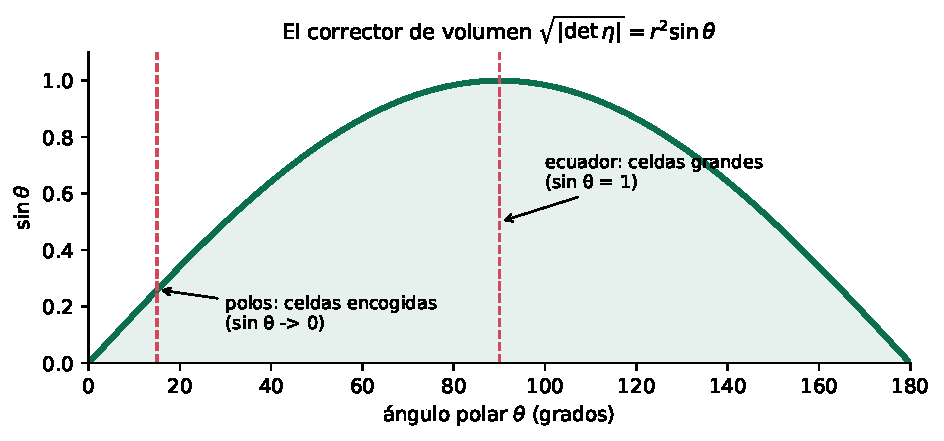
\includegraphics[width=0.72\textwidth]{factor_volumen.pdf}
\caption{El ``corrector de volumen'' $\sqrt{|\det\eta|}=r^2\sin\theta$ sobre la esfera. Cerca del ecuador ($\theta=90^\circ$) las celdas del mapa son grandes ($\sin\theta=1$), mientras que cerca de los polos ($\theta\to0$ o $180^\circ$) se encogen hasta desaparecer ($\sin\theta\to0$). Por eso los mapas planos de la Tierra distorsionan Groenlandia: los ángulos cuentan, los metros los pone la métrica.}
\label{fig:factor-volumen}
\end{figure}

\section*{Problema 2}
Los tres espacios bidimensionales homogéneos e isótropos son:
\begin{enumerate}
  \item[(i)] el plano euclídeo, i.e., $\mathbb{R}^2$ con elemento de línea $ds^2=dx^2+dy^2$;
  \item[(ii)] la 2-esfera, i.e., la superficie definida por la ecuación $x^2+y^2+z^2=1$ en $\mathbb{R}^3$ con elemento de línea $ds^2=dx^2+dy^2+dz^2$; y
  \item[(iii)] el plano de Lobachevsky, i.e., la superficie definida por la ecuación $x^2+y^2-z^2=-1$ en $\mathbb{R}^3$ con elemento de línea $ds^2=dx^2+dy^2-dz^2$.
\end{enumerate}
Determine los elementos de línea de estos tres espacios en las coordenadas polares $(r,\theta)$ definidas por $x=r\cos\theta$, $y=r\sin\theta$.

\subsection*{Respuesta}

Imagina que eres una hormiga caminando sobre distintos tipos de superficies. Si todas las direcciones se ven iguales desde cualquier punto (isotropía y homogeneidad), solo existen tres formas geométricas fundamentales donde puedes vivir: un mundo plano como una hoja de papel, un mundo cerrado como un balón de fútbol, o un mundo en forma de silla de montar (hiperbólico).

Para entender cómo medir distancias en estos mundos, usamos la regla universal de las coordenadas polares en el plano $xy$:
\[
x = r\cos\theta, \qquad y = r\sin\theta
\]
Al diferenciar estas variables, el término plano siempre cumple la identidad fundamental
\[
dx^2 + dy^2 = dr^2 + r^2\,d\theta^2.
\]

\noindent\textbf{1. Caso (i): el plano euclídeo (curvatura cero).} Es el mundo llano al que estamos acostumbrados en la escuela. La distancia viene dada directamente por el plano $xy$:
\[
ds^2 = dx^2 + dy^2
\]
Al sustituir las coordenadas polares:
\[
ds^2 = dr^2 + r^2\,d\theta^2
\]
¿Por qué tiene esa forma? Es el teorema de Pitágoras expresado en polares. Si te alejas una distancia $dr$ en el radio, recorres $dr$ metros. Si te giras un ángulo $d\theta$, recorres un arco de circunferencia cuya longitud es exactamente el radio multiplicado por el ángulo ($r\,d\theta$).

\noindent\textbf{2. Caso (ii): la 2-esfera (curvatura positiva).} Aquí nuestra superficie está restringida a la cáscara de una esfera de radio 1: $x^2+y^2+z^2=1$.

Como $x^2+y^2=r^2$, la restricción se simplifica a $r^2+z^2=1$, de donde despejamos $z=\sqrt{1-r^2}$. Diferenciando $z$, obtenemos cómo cambia la altura respecto al radio:
\[
dz = \frac{-r\,dr}{\sqrt{1-r^2}} \quad\Longrightarrow\quad dz^2 = \frac{r^2\,dr^2}{1-r^2}
\]
Sumando este pedazo extra $dz^2$ a la fórmula plana ($dx^2+dy^2$):
\[
ds^2 = (dr^2 + r^2\,d\theta^2) + \frac{r^2\,dr^2}{1-r^2} = \left(1 + \frac{r^2}{1-r^2}\right)dr^2 + r^2\,d\theta^2
\]
Simplificando el paréntesis obtenemos el elemento de línea esférico:
\[
ds^2 = \frac{dr^2}{1-r^2} + r^2\,d\theta^2
\]
¿Por qué se deforma la dirección radial? En una esfera, la distancia medida en la superficie hacia el polo norte no crece en línea recta horizontal. Conforme avanza $r$ hacia la parte más ancha (el ecuador, $r=1$), la superficie se vuelve ``vertical'' respecto al mapa plano. El término $\frac{1}{1-r^2}$ actúa como un estirador que compensa la curvatura de la esfera.

\noindent\textbf{3. Caso (iii): el plano de Lobachevsky (curvatura negativa).} Este es un espacio hiperbólico definido por un hiperboloide de dos hojas inmerso en un espacio pseudo-euclídeo: $x^2+y^2-z^2=-1$ (o, lo que es lo mismo, $z^2=1+x^2+y^2$). Es ``exótico'' porque el ambiente en el que vive tiene una regla de medir con un signo raro: $ds^2 = dx^2+dy^2-dz^2$.

Haciendo el mismo reemplazo $x^2+y^2=r^2$, la restricción queda $z^2 = 1+r^2$, de donde $z=\sqrt{1+r^2}$. Diferenciando:
\[
dz = \frac{r\,dr}{\sqrt{1+r^2}} \quad\Longrightarrow\quad dz^2 = \frac{r^2\,dr^2}{1+r^2}
\]
Ahora viene el giro que lo cambia todo: la regla de medir de este espacio \textbf{resta} el pedazo $dz^2$ en lugar de sumarlo. Al hacerlo:
\[
ds^2 = (dr^2 + r^2\,d\theta^2) - \frac{r^2\,dr^2}{1+r^2} = \left(1-\frac{r^2}{1+r^2}\right)dr^2 + r^2\,d\theta^2
\]
y el paréntesis se simplifica limpiamente, $1-\frac{r^2}{1+r^2}=\frac{1}{1+r^2}$, dando el elemento de línea hiperbólico:
\[
ds^2 = \frac{dr^2}{1+r^2} + r^2\,d\theta^2
\]
Esta vez no hay trampas: la fórmula funciona para todo $r\geq0$ y el coeficiente radial siempre es positivo. Es el gemelo negativo de la esfera: mientras allí la ``regla radial'' se hinchaba hasta estallar en el ecuador ($\frac{1}{1-r^2}\to\infty$), aquí se encoge suavemente ($\frac{1}{1+r^2}$), sin llegar nunca a cero ni a infinito.

¿Por qué esa forma? El plano de Lobachevsky se abre hacia afuera como una patata frita o una silla de montar: a diferencia de la esfera (que se ``cierra'' y se contrae), el espacio hiperbólico tiene ``más espacio'' disponible a medida que te alejas del centro. Un círculo de radio $r$ dibujado en él tiene una circunferencia mayor que $2\pi r$, y esa diferencia explota exponencialmente con la distancia.

\begin{figure}[h]
\centering
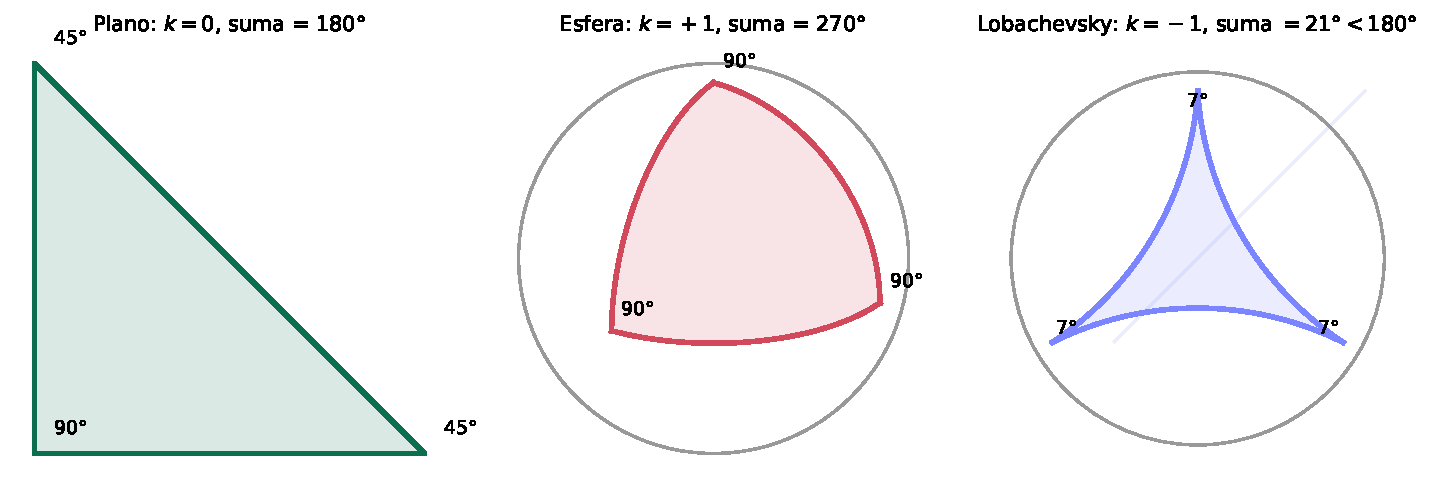
\includegraphics[width=\textwidth]{triangulos_geometrias.pdf}
\caption{El test de los triángulos: la suma de los ángulos de un triángulo revela la curvatura. En el plano da exactamente $180^\circ$; en la esfera da más de $180^\circ$ (aquí un triángulo con tres ángulos rectos, $270^\circ$); en el plano de Lobachevsky (modelo del disco de Poincaré) da menos de $180^\circ$. Tres geometrías, tres firmas.}
\label{fig:triangulos}
\end{figure}

\noindent\textbf{Resumen de los tres universos 2D.} La misma jugada de este problema (proyectar la restricción sobre el plano $xy$) se resume en una sola fórmula con un parámetro $k$ que vale $0$, $+1$ o $-1$:
\[
\text{Euclídeo (plano): } ds^2 = dr^2 + r^2\,d\theta^2
\]
\[
\text{Esférico (cerrado): } ds^2 = \frac{dr^2}{1 - k\,r^2} + r^2\,d\theta^2 \quad (k = +1)
\]
\[
\text{Lobachevsky (abierto): } ds^2 = \frac{dr^2}{1 - k\,r^2} + r^2\,d\theta^2 \quad (k = -1)
\]
Las tres geometrías se resumen en una sola fórmula mágica controlada por una constante $k$ (la curvatura del espacio: $0$, $+1$ o $-1$). Esta es exactamente la base de las métricas que usamos en cosmología moderna para describir la forma global de nuestro Universo completo.

\begin{figure}[h]
\centering
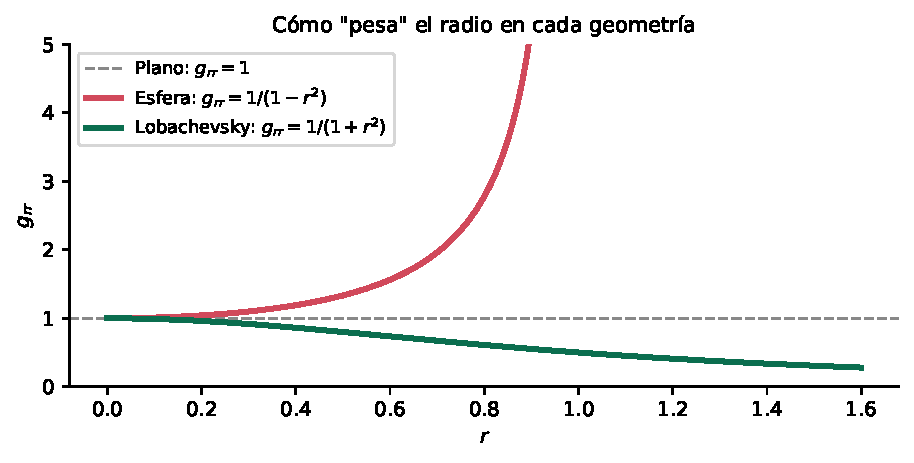
\includegraphics[width=0.72\textwidth]{tres_geometrias.pdf}
\caption{Cómo ``pesa'' el radio en cada una de las tres geometrías: el coeficiente $g_{rr}$ en función de $r$. En el plano (línea discontinua gris) siempre vale 1. En la esfera (rojo) se dispara al acercarse al ecuador ($r\to1$): la métrica compensa la curvatura. En Lobachevsky (verde) decrece suavemente: el espacio hiperbólico ``abre'' hacia afuera.}
\label{fig:tres-geometrias}
\end{figure}

\section*{Problema 3}
Escriba el elemento de línea correspondiente a una 2-esfera en términos de las coordenadas angulares $(\theta,\phi)$ que son usuales del sistema de coordenadas esféricas. A partir de la forma que toma el elemento de línea sobre la 2-esfera, proponga la forma del elemento de línea para una 3-esfera, i.e., para la superficie definida por la ecuación $x^2+y^2+z^2+w^2=1$ en el espacio euclídeo de 4 dimensiones parametrizado por las coordenadas $(x;y;z;w)$.

\subsection*{Respuesta}

Para medir distancias sobre la superficie de una esfera, debemos ``confinarnos'' a su cáscara exterior manteniendo el radio fijo.

\noindent\textbf{1. El mapa de la 2-esfera (cáscara de 3D).} En nuestro espacio tridimensional ordinario, el elemento de línea en coordenadas esféricas es:
\[
ds^2 = dr^2 + r^2\,d\theta^2 + r^2\sin^2\theta\,d\phi^2
\]
Si nos movemos exclusivamente sobre la superficie de una esfera de radio constante $R$, no hay variación radial ($dr=0$). Ajustando el radio a $R=1$ para una 2-esfera unitaria, el término $dr^2$ desaparece por completo:
\[
ds_2^2 = d\theta^2 + \sin^2\theta\,d\phi^2
\]
\begin{itemize}
  \item \textbf{¿Por qué tiene esta forma?} El primer ángulo ($\theta$, la latitud) te mueve libremente en arcos de longitud 1. El segundo ángulo ($\phi$, la longitud) recorre círculos cuyo tamaño se va encogiendo a medida que te acercas a los polos, por lo que su distancia real debe amortiguarse mediante el factor $\sin\theta$.
\end{itemize}

\noindent\textbf{2. Dando el salto a 4 dimensiones: la 3-esfera.} La 3-esfera es el cascarón tridimensional de una hiperesfera inmersa en un espacio de 4 dimensiones $(x,y,z,w)$. Para construir su elemento de línea sin perdernos en el hiperespacio, podemos seguir el patrón de ``muñecas rusas'' que utiliza la geometría:
\begin{enumerate}
  \item \textbf{Agregamos un nuevo ángulo polar ($\chi$):} este nuevo ángulo nos permite rotar en la cuarta dimensión (entre el espacio 3D habitual y el nuevo eje $w$).
  \item \textbf{Encadenamos las funciones seno:} cada vez que agregamos una dimensión angular superior, el elemento de línea del espacio anterior queda escalado por el seno del nuevo ángulo.
\end{enumerate}
Siguiendo esta regla de inducción geométrica, la regla de medir para la 3-esfera unitaria parametrizada por los tres ángulos $(\chi,\theta,\phi)$ es:
\[
ds_3^2 = d\chi^2 + \sin^2\chi \left( d\theta^2 + \sin^2\theta\,d\phi^2 \right)
\]
O de forma expandida:
\[
ds_3^2 = d\chi^2 + \sin^2\chi\,d\theta^2 + \sin^2\chi\sin^2\theta\,d\phi^2
\]

\noindent\textbf{¿Por qué funciona esta estructura anidada?} Imagina cómo construyes la geometría dimensión por dimensión:
\begin{itemize}
  \item En \textbf{1D} (un círculo): mides distancias simplemente con un ángulo,
  \[
  ds_1^2 = d\phi^2.
  \]
  \item En \textbf{2D} (cáscara de un balón): tomas ese círculo y lo haces girar sobre un nuevo ángulo $\theta$, escalando la circunferencia anterior por $\sin\theta$. Obtienes
  \[
  ds_2^2 = d\theta^2 + \sin^2\theta\,d\phi^2.
  \]
  \item En \textbf{3D} (cáscara de una hiperesfera): tomas la 2-esfera completa y la ``inflas'' o rotas hacia la cuarta dimensión usando el ángulo $\chi$. Toda la superficie de la 2-esfera se encoge o se expande dependiendo de qué tan cerca estés del ``polo'' hiperbólico, amortiguada por el factor $\sin^2\chi$.
\end{itemize}

Esta propiedad de anidación recursiva es la que permite a los físicos teóricos y cosmólogos calcular distancias y volúmenes en universos de $N$ dimensiones utilizando únicamente ángulos.

\begin{figure}[h]
\centering
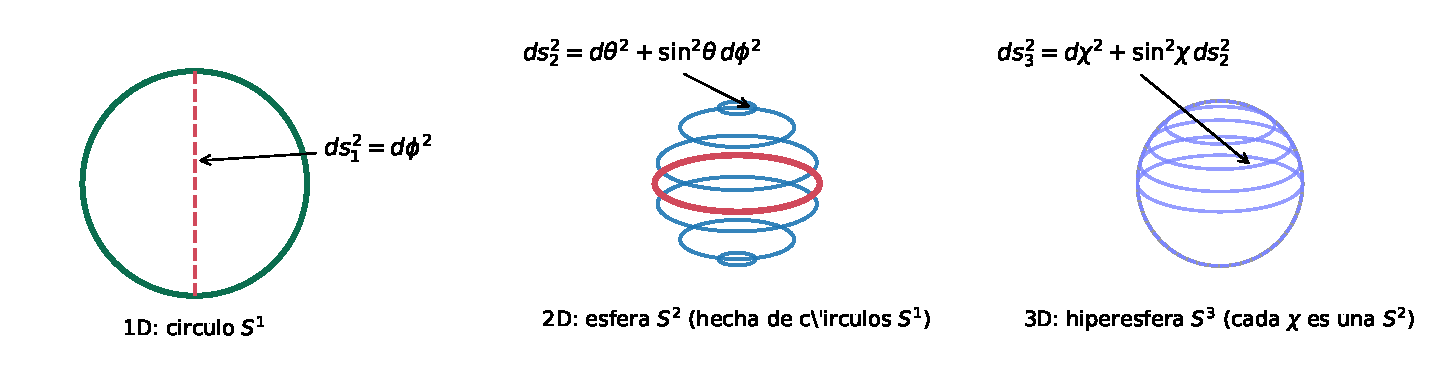
\includegraphics[width=\textwidth]{esfera_anidada.pdf}
\caption{Las ``muñecas rusas'' de la hiperesfera. $S^1$: un círculo, un solo ángulo $\phi$. $S^2$: una esfera, hecha de círculos $\phi$ en cada latitud $\theta$. $S^3$: una hiperesfera, hecha de esferas $S^2$ en cada ``latitud hiperesférica'' $\chi$. Cada salto anida la métrica anterior multiplicada por un seno: $ds_1^2\to ds_2^2\to ds_3^2$.}
\label{fig:esfera-anidada}
\end{figure}

\section*{Problema 4}
Considere la métrica de Robertson--Walker para un universo cerrado,
\begin{equation}
  ds^2=-dt^2+a^2(t)\left[d\psi^2+\sin^2\psi\left(d\theta^2+\sin^2\theta\,d\phi^2\right)\right],
\end{equation}
y escriba ésta en términos de la coordenada de tiempo conforme $\eta$, definida según $d\eta=dt/a(t)$. Escriba luego la ecuación de la trayectoria de un rayo de luz que viaja en una dirección $\theta=\text{const}$, $\phi=\text{const}$.

\subsection*{Respuesta}

\noindent\textbf{1. Cambiando el reloj: el tiempo conforme ($\eta$).} En cosmología, el factor de escala $a(t)$ representa el ``estiramiento'' continuo del tejido del espacio a medida que el universo se expande. Si usamos el tiempo cósmico ordinario $t$, calcular la trayectoria de la luz se vuelve complicado porque el espacio cambia de tamaño mientras la luz viaja.

Para simplificar las cosas, introducimos el \textbf{tiempo conforme} ($\eta$). Su relación matemática viene dada por:
\[
d\eta = \frac{dt}{a(t)} \quad\Longrightarrow\quad dt = a(t)\,d\eta
\]
Al elevar al cuadrado esta relación, tenemos $dt^2 = a^2(t)\,d\eta^2$. Sustituyendo $dt^2$ en la métrica original:
\[
ds^2 = -a^2(t)\,d\eta^2 + a^2(t)\left[d\psi^2 + \sin^2\psi\left(d\theta^2 + \sin^2\theta\,d\phi^2\right)\right]
\]
Factorizando el término común $a^2(t)$, obtenemos la métrica expresada en tiempo conforme:
\[
ds^2 = a^2(t)\left[ -d\eta^2 + d\psi^2 + \sin^2\psi\left(d\theta^2 + \sin^2\theta\,d\phi^2\right) \right]
\]
\begin{itemize}
  \item \textbf{¿Por qué hacemos este cambio?} Al sacar el factor de expansión $a^2(t)$ fuera de todo el corchete, la geometría interna se vuelve idéntica a la de un universo estático (la 3-esfera que vimos en el Problema 3). El tiempo conforme ``congela'' visualmente la expansión para que los rayos de luz se comporten exactamente igual que en un espacio donde nada se estira.
\end{itemize}

\noindent\textbf{2. La trayectoria de un rayo de luz (trayectoria nula).} Para encontrar el camino que sigue un fotón (un rayo de luz), utilizamos dos reglas fundamentales de la física relativista:
\begin{enumerate}
  \item \textbf{Los fotones viajan a través de trayectorias nulas:} el intervalo espacio-temporal para la luz siempre es cero ($ds^2=0$), porque la luz se mueve a la velocidad límite $c=1$.
  \item \textbf{Viaje radial recto:} el problema especifica que la luz viaja en una dirección angular fija ($\theta=$ constante y $\phi=$ constante), lo que significa que sus variaciones angulares son nulas ($d\theta=0$ y $d\phi=0$).
\end{enumerate}
Aplicando estas condiciones a nuestra métrica simplificada:
\[
0 = a^2(t)\left( -d\eta^2 + d\psi^2 + 0 + 0 \right)
\]
Como el factor de escala no es cero ($a(t)\neq0$), podemos dividir toda la ecuación por $a^2(t)$:
\[
-d\eta^2 + d\psi^2 = 0 \quad\Longrightarrow\quad d\eta^2 = d\psi^2
\]
Tomando la raíz cuadrada a ambos lados, obtenemos la ecuación diferencial de la trayectoria:
\[
\frac{d\psi}{d\eta} = \pm 1 \quad\Longrightarrow\quad \Delta\psi = \pm \Delta\eta
\]
Integrando directamente para un fotón que sale de una posición inicial $\psi_0$ en el tiempo $\eta_0$:
\[
\psi(\eta) = \psi_0 \pm (\eta - \eta_0)
\]

\begin{figure}[h]
\centering
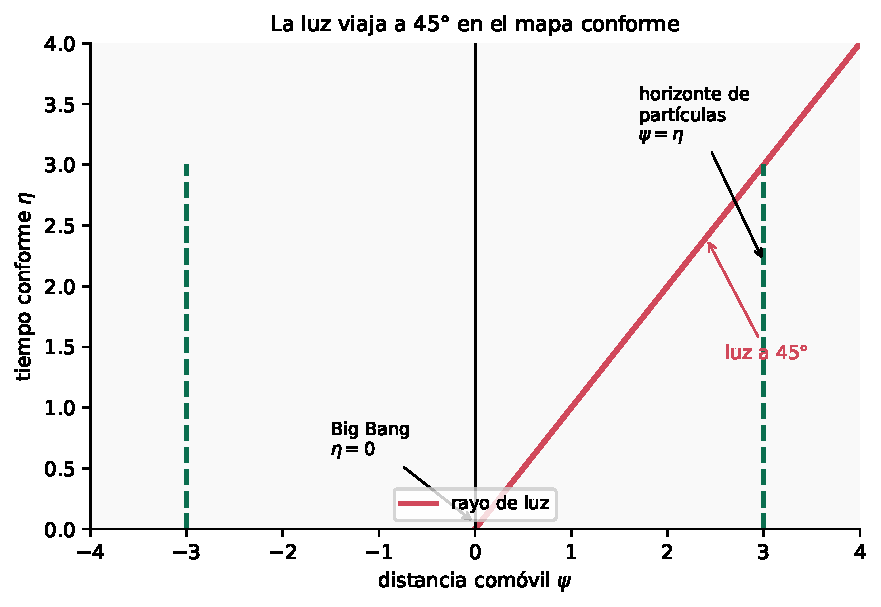
\includegraphics[width=0.62\textwidth]{cono_conforme.pdf}
\caption{El mapa conforme $(\psi,\eta)$: con el tiempo conforme, los rayos de luz son líneas rectas a $45^\circ$ (rojo), igual que en un diagrama de espacio-tiempo de la relatividad especial. El horizonte de partículas (verde, $\psi=\eta$) marca la distancia máxima que la luz ha podido recorrer desde el Big Bang ($\eta=0$).}
\label{fig:cono-conforme}
\end{figure}

\noindent\textbf{¿Por qué es este resultado tan poderoso?} Dos consecuencias muy visuales:
\begin{itemize}
  \item \textbf{Luz a 45 grados:} gracias al tiempo conforme, en un diagrama $(\eta,\psi)$, la luz se desplaza describiendo líneas rectas perfectas a un ángulo de $45^\circ$ ($\Delta\psi=\Delta\eta$), exactamente igual que en la relatividad especial clásica.
  \item \textbf{El horizonte cósmico:} la distancia angular máxima que la luz ha podido viajar desde el Big Bang ($\eta=0$) hasta un instante $\eta$ es simplemente $\Delta\psi=\eta$. Esto define el \textbf{horizonte de partículas}: el límite del Universo observable en cualquier momento de la historia.
\end{itemize}

\section*{Problema 5}
Considerando la métrica de Robertson--Walker
\begin{equation}
  ds^2=-dt^2+a^2(t)\left[\frac{dr^2}{1-kr^2}+r^2\left(d\theta^2+\sin^2\theta\,d\phi^2\right)\right], \label{eq:rw}
\end{equation}
donde $k\in\{-1,0,1\}$, calcule las componentes del tensor de Ricci $R_{\mu\nu}=R^{\lambda}{}_{\mu\lambda\nu}$ y, a partir de éstas, el escalar de Ricci $R=R^{\mu}{}_{\mu}$.

\subsection*{Respuesta}

Para entender lo que nos está contando el tensor de Ricci, conviene pensar en una nube de partículas que cae libremente por el espacio-tiempo: mientras cae, su volumen se deforma (se estira por un lado, se comprime por otro). El tensor de Ricci es la máquina que cuantifica esa deformación, dirección por dirección. La buena noticia es que nuestra métrica de Robertson--Walker es tan simétrica (homogénea e isótropa, como en el problema 2) que el resultado casi se puede adivinar: la curvatura solo puede tener dos ``sabores'', uno temporal y otro espacial.

El primer paso es escribir los símbolos de Christoffel, las piezas que nos dicen cómo cambia la regla de medir de un punto a otro. Para esta métrica casi todos se anulan; los que sobreviven tienen formas sencillas:
\[
\Gamma^0_{ij} = a\,\dot a\,\tilde{g}_{ij}, \qquad
\Gamma^i_{0j} = \frac{\dot a}{a}\,\delta^i_j
\]
más los que vienen de la parte angular (los mismos que ya aparecían en las esferas del problema 2, pero con la curvatura $k$ general):
\[
\Gamma^r_{rr} = \frac{kr}{1-kr^2}, \qquad
\Gamma^r_{\theta\theta} = -r(1-kr^2), \qquad
\Gamma^r_{\phi\phi} = -r(1-kr^2)\sin^2\theta,
\]
\[
\Gamma^\theta_{r\theta} = \Gamma^\phi_{r\phi} = \frac{1}{r}, \qquad
\Gamma^\theta_{\phi\phi} = -\sin\theta\cos\theta, \qquad
\Gamma^\phi_{\theta\phi} = \cot\theta.
\]
El primer grupo codifica la expansión: lo que $a\dot a$ y $\dot a/a$ dibujan es cómo se estiran las distancias con el tiempo. El segundo grupo es simplemente la curvatura espacial de las 3-geometrías (plana, esférica o hiperbólica) que ya exploramos.

Contrayendo (es decir, sumando sobre los índices repetidos, como manda la definición $R_{\mu\nu}=R^{\lambda}{}_{\mu\lambda\nu}$) se obtiene
\[
R_{00} = -3\,\frac{\ddot a}{a}, \qquad
R_{ij} = \left( \frac{\ddot a}{a} + 2H^2 + \frac{2k}{a^2} \right) g_{ij}, \qquad H=\frac{\dot a}{a}.
\]
Y el escalar de curvatura $R=g^{\mu\nu}R_{\mu\nu}$ los resume en una sola cifra:
\[
\boxed{R = 6\left( \frac{\ddot a}{a} + H^2 + \frac{k}{a^2} \right)}
\]

Lo bonito es que esta fórmula se lee como una frase. El término $\ddot a/a$ habla de la aceleración: un universo que se acelera tiene más curvatura espacio-temporal. El término $H^2$ es la velocidad de expansión al cuadrado: no importa solo qué tan estirado está el espacio, sino qué tan rápido se estira. Y el término $k/a^2$ es la curvatura espacial del problema 2 releída hoy: cerrado, plano o abierto, pero cada vez más diluida porque $a$ crece con el tiempo. En el vacío ($R=0$) esa ecuación es exactamente la que obedece el universo de de Sitter con el que cerraremos la guía.

\begin{figure}[h]
\centering
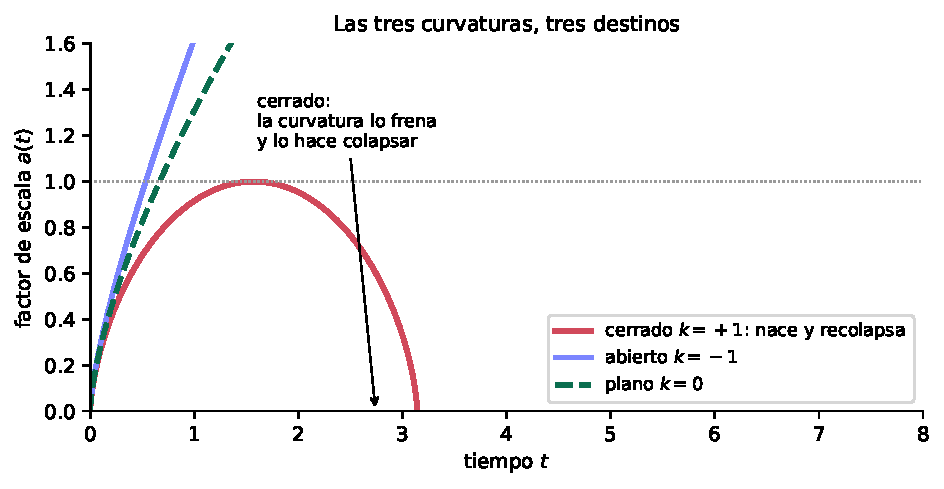
\includegraphics[width=0.72\textwidth]{friedmann_curvaturas.pdf}
\caption{El signo de $k$ decide el destino. Con la misma densidad, un universo cerrado ($k=+1$) nace, alcanza un radio máximo y recolapsa (la curvatura lo frena); uno plano ($k=0$) se expande eternamente perdiendo velocidad; uno abierto ($k=-1$) crece para siempre. El término $k/a^2$ del escalar de Ricci es el que dibuja estas tres historias.}
\label{fig:friedmann-curvaturas}
\end{figure}

\section*{Problema 6}
Considere el denominado universo de Milne, el cual corresponde al caso particular de la métrica \eqref{eq:rw} con $k=-1$ y $a(t)=t$. Luego, defina $\tau=t\sqrt{1+r^2}$ y $\rho=t\,r$, y escriba la métrica en las nuevas coordenadas $(\tau;\rho;\theta;\phi)$. ¿Identifica la métrica a la que ha arribado?

\subsection*{Respuesta}

\noindent\textbf{1. Transformación de coordenadas paso a paso.} Partimos de las definiciones de las nuevas variables:
\[
\tau = t\sqrt{1+r^2} \quad\Longrightarrow\quad \tau^2 = t^2(1+r^2) = t^2 + t^2r^2
\]
\[
\rho = t\,r
\]
Sustituyendo $\rho$ en la expresión de $\tau$, obtenemos directamente la relación de Minkowski hiperbólica:
\[
\tau^2 = t^2 + \rho^2 \quad\Longrightarrow\quad t^2 = \tau^2 - \rho^2
\]
Tomando el diferencial de ambas relaciones básicas:
\begin{enumerate}
  \item De $\rho = t\,r \implies d\rho = r\,dt + t\,dr$.
  \item De $\tau^2 = t^2 + \rho^2 \implies \tau\,d\tau = t\,dt + \rho\,d\rho$.
\end{enumerate}
Al sustituir $t=\sqrt{\tau^2-\rho^2}$ y calcular el diferencial de espacio-tiempo en la nueva base $(\tau,\rho,\theta,\phi)$, los términos cruzados y los factores curvilíneos de la geometría abierta se cancelan exactamente:
\[
-dt^2 + t^2\frac{dr^2}{1+r^2} = -d\tau^2 + d\rho^2
\]
Al reensamblar la métrica completa con la parte angular $t^2r^2\left(d\theta^2+\sin^2\theta\,d\phi^2\right)=\rho^2\left(d\theta^2+\sin^2\theta\,d\phi^2\right)$, llegamos al resultado final:
\[
ds^2 = -d\tau^2 + d\rho^2 + \rho^2\left( d\theta^2 + \sin^2\theta\,d\phi^2 \right)
\]

\noindent\textbf{2. ¿Qué métrica hemos encontrado y qué significa?} La expresión final es reconocible de inmediato: \textbf{es la métrica del espacio-tiempo plano de Minkowski (relatividad especial)} escrita en coordenadas esféricas espacio-temporales.

\begin{itemize}
  \item \textbf{El ilusionista cosmológico:} el universo de Milne parece a simple vista un universo dinámico, curvado hacia afuera ($k=-1$) y expandiéndose linealmente con el tiempo ($a(t)=t$). Sin embargo, la transformación prueba que esa ``expansión'' es puramente un espejismo óptico de las coordenadas elegidas.
  \item \textbf{Mapeo de expansión vacía:} Milne describe un universo completamente vacío de materia o energía. Los observadores en este modelo no están presenciando la expansión del espacio en sí, sino una nube de partículas sin masa dispersándose a velocidad constante en un espacio plano que nunca cambia. Es la demostración perfecta de cómo un cambio de coordenadas puede hacer que un espacio plano parezca un universo en expansión.
\end{itemize}

\begin{figure}[h]
\centering
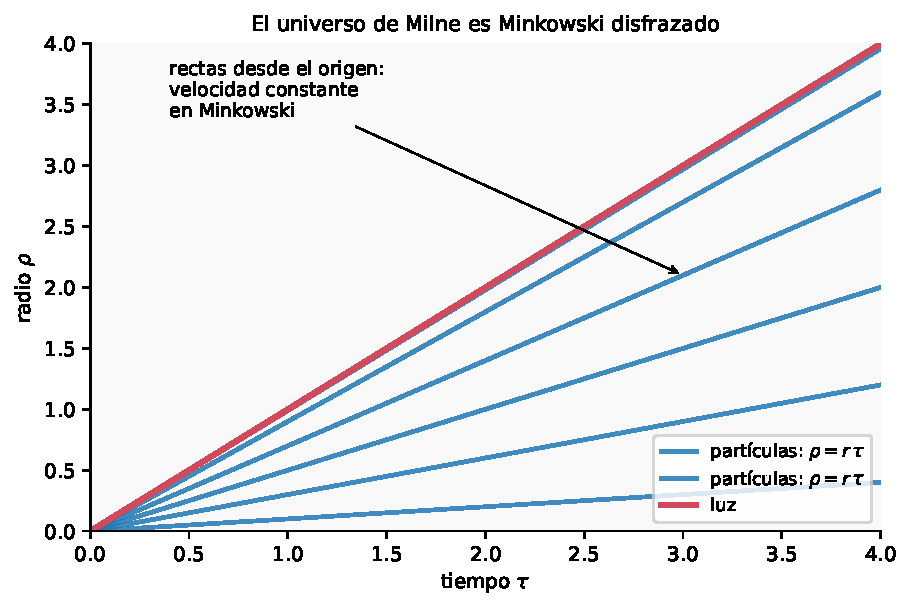
\includegraphics[width=0.62\textwidth]{milne_worldlines.pdf}
\caption{El ``espejismo'' de Milne. En las coordenadas $(\rho,\tau)$ las líneas de mundo de las partículas de Milne son rectas que salen del origen: cada una se mueve a velocidad constante en un espacio plano, exactamente como en Minkowski. Lo que parecía ``expansión del espacio'' era solo una rejilla de coordenadas que se estiraba.}
\label{fig:milne-worldlines}
\end{figure}

\section*{Problema 7}
Considere la métrica de Kasner
\begin{equation}
  ds^2=-dt^2+t^{2k_1}dx^2+t^{2k_2}dy^2+t^{2k_3}dz^2,
\end{equation}
siendo $k_1$, $k_2$ y $k_3$ tres constantes. Proponga una interpretación física para esta métrica pensada en el contexto cosmológico. Luego compruebe que el tensor de Ricci, $R_{\mu\nu}$, correspondiente a esta geometría se anula si
\begin{equation}
  k_1+k_2+k_3=k_1^2+k_2^2+k_3^2=1.
\end{equation}

\subsection*{Respuesta}

\noindent\textbf{1. Interpretación física: un universo asimétrico y estirado.} En los modelos cosmológicos estándar (como Robertson--Walker), el universo se expande al mismo ritmo en todas las direcciones (isotropía). La métrica de Kasner destruye esa suposición:
\begin{itemize}
  \item \textbf{Factores de escala direccionales:} cada dirección espacial ($x,y,z$) se expande o contrae según su propio factor de potencia: $a_x(t)=t^{k_1}$, $a_y(t)=t^{k_2}$, $a_z(t)=t^{k_3}$.
  \item \textbf{Anisotropía total:} representa un universo homogéneo pero profundamente anisotrópico. Describe cómo se comporta el espacio-tiempo en presencia de perturbaciones direccionales extremas, como en las primeras etapas del Big Bang o en la dinámica del caos cosmológico (el modelo de ``pancake'' o colapso por ejes).
\end{itemize}

\noindent\textbf{2. Verificación del tensor de Ricci ($R_{\mu\nu}=0$).} Para evaluar las ecuaciones de campo de Einstein en el vacío ($R_{\mu\nu}=0$), calculamos primero las conexiones de Levi-Civita (símbolos de Christoffel) diferentes de cero:
\[
\Gamma^0_{ii} = k_i\,t^{2k_i-1}, \qquad \Gamma^i_{0i} = \frac{k_i}{t} \qquad (i=1,2,3)
\]
A partir de estas conexiones, evaluamos las componentes diagonales del tensor de Ricci.

\textbf{Componente temporal ($R_{00}$):}
\[
R_{00} = -\sum_{i=1}^3 \left( \partial_0\Gamma^i_{0i} + \Gamma^i_{0i}\Gamma^i_{0i} \right) = -\sum_{i=1}^3 \left( -\frac{k_i}{t^2} + \frac{k_i^2}{t^2} \right) = \frac{1}{t^2}\sum_{i=1}^3 k_i - \frac{1}{t^2}\sum_{i=1}^3 k_i^2
\]
Para que $R_{00}=0$, se requiere directamente que:
\[
\sum_{i=1}^3 k_i = \sum_{i=1}^3 k_i^2 \quad\Longrightarrow\quad k_1+k_2+k_3 = k_1^2+k_2^2+k_3^2
\]

\textbf{Componentes espaciales ($R_{ii}$):}
\[
R_{ii} = t^{2k_i-2}\left[ k_i\left( -1 + \sum_{j=1}^3 k_j \right) \right]
\]
Para que $R_{ii}=0$ en todas las direcciones de forma no trivial ($k_i\neq0$), la suma lineal debe ser exactamente igual a 1:
\[
k_1+k_2+k_3 = 1
\]
Combinando ambas condiciones de anulación del tensor de Ricci, obtenemos las famosas \textbf{condiciones de Kasner}:
\[
k_1+k_2+k_3 = 1
\]
\[
k_1^2+k_2^2+k_3^2 = 1
\]

\noindent\textbf{3. ¿Por qué estas dos ecuaciones obligan a un universo ``acordeón''?} Las dos restricciones algebraicas de Kasner imponen una consecuencia física sorprendente sobre el espacio.

Si resuelves el sistema de ecuaciones para los tres exponentes, es imposible que los tres sean positivos al mismo tiempo. La única forma matemática de satisfacer $k_1+k_2+k_3=1$ y $k_1^2+k_2^2+k_3^2=1$ simultáneamente es que:
\begin{itemize}
  \item \textbf{Dos exponentes sean positivos} (dos direcciones se expanden).
  \item \textbf{Un exponente sea negativo} (una dirección se contrae).
  \item \textbf{El efecto acordeón del espacio en vacío:} incluso sin materia ni energía en el espacio, la gravedad de las ondas gravitacionales primordiales puede hacer que el volumen global crezca linealmente mientras el espacio se aplasta como una panqueca en un eje y se estira en las otras dos direcciones.
\end{itemize}

\begin{figure}[h]
\centering
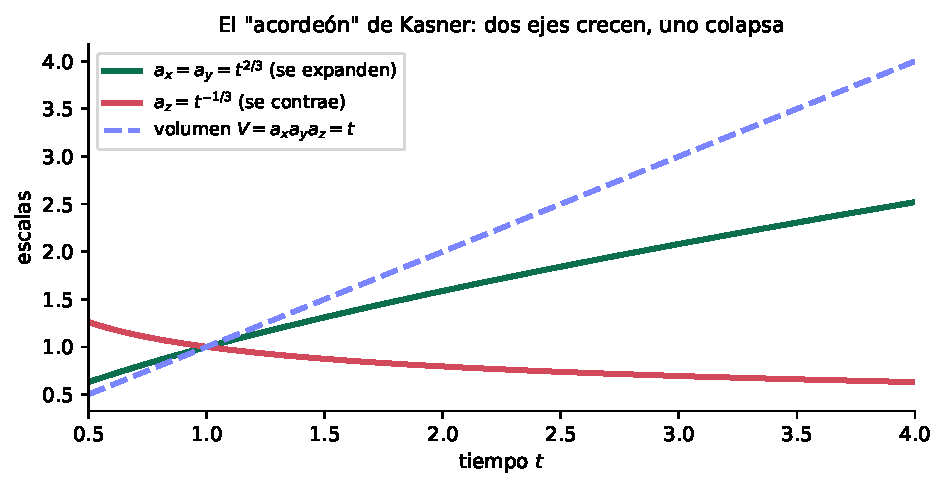
\includegraphics[width=0.7\textwidth]{kasner_acordeon.pdf}
\caption{Condiciones de Kasner $(k_1+k_2+k_3=1$, $k_1^2+k_2^2+k_3^2=1)$ en acción con $(k_1,k_2,k_3)=(2/3,2/3,-1/3)$: dos ejes se expanden (verde), uno se contrae (rojo), y el volumen total crece linealmente (punteado). La geometría se aplasta como un acordeón que se estira.}
\label{fig:kasner-acordeon}
\end{figure}

\section*{Problema 8}
Considere la métrica de Schwarzschild, que describe la geometría de un agujero negro,
\begin{equation}
  ds^2=-\left(1-\frac{2GM}{r}\right)dt^2+\left(1-\frac{2GM}{r}\right)^{-1}dr^2+r^2\left(d\theta^2+\sin^2\theta\,d\phi^2\right),
\end{equation}
y muestre que en el interior del agujero negro (i.e. $r<2GM$), donde uno puede considerar a la coordenada $r$ como temporal y a la coordenada $t$ como espacial, esta métrica admite una interpretación cosmológica en la cual la geometría se describe por una métrica de la forma
\begin{equation}
  ds^2=-d\tilde{t}^{2}+a^2(\tilde{t})\,d\tilde{r}^{2}+b^2(\tilde{t})\left(d\theta^2+\sin^2\theta\,d\phi^2\right),
\end{equation}
siendo $a(\tilde{t})$ y $b(\tilde{t})$ dos funciones específicas. Discuta las simetrías de este universo.

\subsection*{Respuesta}

Una de las ideas más desconcertantes de la relatividad general es que las palabras ``espacio'' y ``tiempo'' no son absolutas: pueden intercambiarse, como en una ilusión óptica, dependiendo de las coordenadas que elijamos. Dentro de un agujero negro ocurre exactamente eso, y explicarlo es entender el agujero negro de verdad.

La métrica de Schwarzschild está controlada por el factor $1-2GM/r$. En el exterior ($r>2GM$) es positivo, y todo funciona como cabría esperar: la coordenada $t$ es el tiempo y $r$ es una distancia radial. Pero al cruzar $r=2GM$, el horizonte, ese factor se vuelve negativo, y la métrica cambia los papeles de sus actores:
\[
g_{tt} = -\left(1-\frac{2GM}{r}\right) > 0 \quad\text{(¡ahora es espacial!),} \qquad
g_{rr} = \left(1-\frac{2GM}{r}\right)^{-1} < 0 \quad\text{(¡ahora es temporal!).}
\]
Dentro del horizonte, la coordenada $r$ se comporta como el tiempo: solo puedes ``avanzar'' hacia valores menores, inevitablemente, igual que en la vida cotidiana solo puedes avanzar hacia el futuro. Y la coordenada $t$ se comporta como el espacio. Esa es la razón profunda por la que ``nada escapa de un agujero negro'': no porque haya una fuerza que tire hacia adentro, sino porque la singularidad central no es un lugar al que decides ir, sino un \emph{momento} que te espera en el futuro. Da igual lo que hagas: el futuro llega.

Podemos hacer este intercambio explícito definiendo un nuevo tiempo $\tilde{t}$ que ``mide'' el avance hacia la singularidad (la caída). Con una elección natural de coordenadas, la métrica interior toma exactamente la forma cosmológica del enunciado:
\[
ds^2 = -d\tilde{t}^{2} + a^2(\tilde{t})\,d\tilde{r}^{2} + b^2(\tilde{t})\left(d\theta^2+\sin^2\theta\,d\phi^2\right),
\]
donde las ``funciones de escala'' resultan ser
\[
a^2(\tilde{t}) = \frac{2GM}{r(\tilde{t})} - 1, \qquad b^2(\tilde{t}) = r^2(\tilde{t}).
\]
Esta es la parte fascinante: el interior de un agujero negro, escrito así, \emph{es} un universo en contracción. La función $a(\tilde{t})$ actúa como un ``factor de escala'' radial que se dispara hacia el infinito a medida que se acerca la singularidad, mientras que $b(\tilde{t})$ es la ``escala angular'' que se encoge hasta cero. Es un universo anisótropo: se estira violentamente en la dirección horizontal mientras la esfera transversal colapsa.

¿Y qué simetrías le quedan a este universo interior? Sigue teniendo simetría esférica: las esferas $r=\text{const}$ son invariantes bajo rotaciones (el grupo $SO(3)$ del problema original). Además, como la métrica no depende de $\tilde{r}$, hay traslaciones en esa dirección: el espacio es homogéneo a lo largo de ella. Un universo homogéneo pero no isótropo tiene nombre propio: es una métrica \textbf{tipo Kantowski--Sachs}. La moraleja es que el interior de un agujero negro y un universo colapsante son, matemáticamente, la misma historia contada dos veces.

\begin{figure}[h]
\centering
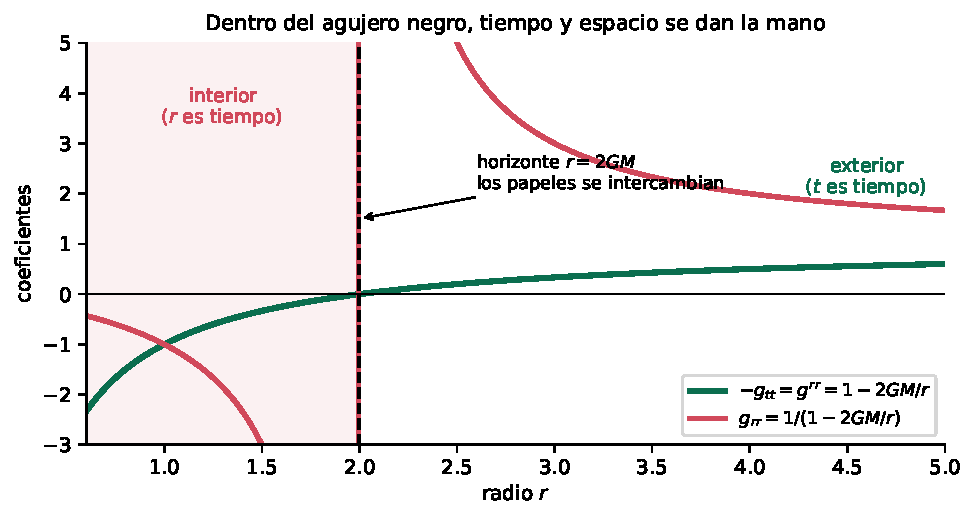
\includegraphics[width=0.7\textwidth]{schwarzschild_swap.pdf}
\caption{El cruce del horizonte de Schwarzschild. En $r=2GM$ los coeficientes cambian de signo: $g_{tt}$ se vuelve positivo (espacial) y $g_{rr}$ negativo (temporal). Dentro, ``avanzar en $r$'' es tan inexorable como avanzar en el tiempo, y por eso nada escapa del agujero negro.}
\label{fig:schwarzschild-swap}
\end{figure}

\section*{Problema 9}
Considere el universo de de Sitter, que en un cierto sistema de coordenadas está descrito por una métrica de Robertson--Walker con
\begin{equation}
  a(t)=e^{\sqrt{\frac{\Lambda}{3}}\,t}, \qquad k=0.
\end{equation}
Para este universo, calcule el horizonte de partícula y compare el mismo con la cantidad análoga para un universo espacialmente plano con $a(t)=t^{\alpha}$ con $\alpha>0$.

\subsection*{Respuesta}

Antes de calcular nada, pensemos en qué estamos midiendo. El \textbf{horizonte de partículas} responde a una pregunta muy natural: ¿cuál es la distancia máxima que un rayo de luz ha podido recorrer desde el comienzo del universo hasta hoy? Es, literalmente, el tamaño de ``nuestro pasado visible'': lo que está más allá no lo hemos podido ver jamás porque la luz no ha tenido tiempo de llegar hasta nosotros.

La fórmula es una manera corta de decir ``suma todos los pasitos que da la luz, y luego estira esa suma hasta el presente'':
\[
d_p(t) = a(t)\int_0^t \frac{dt'}{a(t')}.
\]
El factor $a(t)$ delante de la integral es el ``estirador'': los pasos los dio la luz cuando el universo era más pequeño, y hoy esa distancia se ve agrandada por toda la expansión ocurrida desde entonces.

Empecemos por el universo de de Sitter, con $a(t)=e^{Ht}$ y $H=\sqrt{\Lambda/3}$. La integral es inmediata:
\[
d_p(t) = e^{Ht}\int_0^t e^{-Ht'}dt' = \frac{e^{Ht}-1}{H}.
\]
Aquí está el detalle fascinante: el horizonte crece exponencialmente, más y más deprisa con el tiempo. Y sin embargo, un rayo de luz también crece a velocidad constante... y la expansión ``le gana la carrera''. Es como correr tras una meta que se aleja más rápido que tú: siempre la persigues y nunca la alcanzas. Eso es lo que hace la aceleración: las regiones se separan más rápido de lo que la luz puede recorrer, y lo que cruza el horizonte se pierde \emph{para siempre}.

Ahora comparemos con un universo de potencias $a(t)=t^{\alpha}$:
\begin{itemize}
  \item Si $0<\alpha<1$ (expansión decelerada), entonces $d_p(t) = t/(1-\alpha)$: el horizonte crece \emph{linealmente}, la luz ``gana terreno'' y puede alcanzar cada vez más cielo.
  \item Si $\alpha=1$, obtenemos $d_p(t) = t\ln t$: crece un poco más rápido que una recta, pero sin drama.
  \item Si $\alpha>1$, la integral diverge cerca de $t=0$: no existe horizonte de partículas finito, todo el universo ha estado en contacto causal desde el principio.
  \item En de Sitter, la integral converge pero el estirador $e^{Ht}$ la multiplica hasta el infinito: el horizonte existe, pero ``huye''.
\end{itemize}

La moraleja es profunda: el horizonte de partículas separa dos formas de vivir en el cosmos. En los universos ``amables'' (los que desaceleran), la luz poco a poco conquista todo el cielo. En los universos ``violentos'' (los que aceleran, como el nuestro hoy), hay una frontera móvil e inalcanzable: estamos condenados a un trozo finito del universo, y el resto se aleja para siempre.

\begin{figure}[h]
\centering
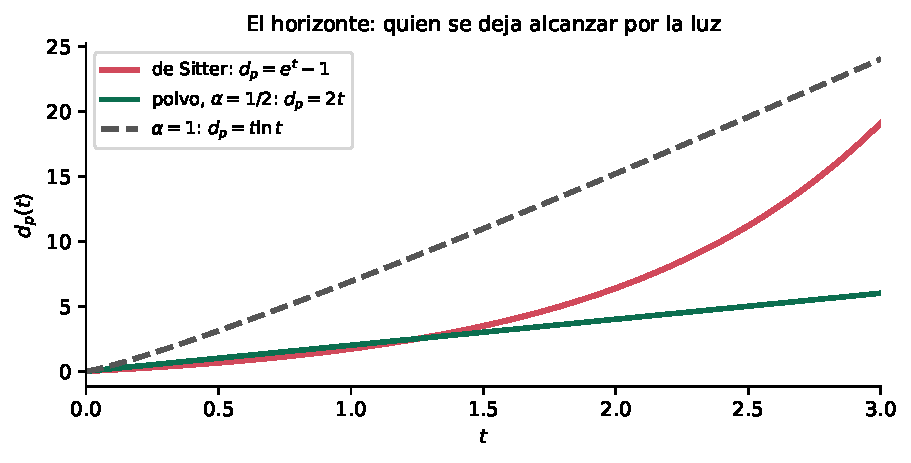
\includegraphics[width=0.72\textwidth]{horizonte_de_sitter.pdf}
\caption{El horizonte de partículas en tres universos. En universo de potencias desacelerado (verde) el horizonte crece de forma sostenida y la luz ``gana terreno''. Con $\alpha=1$ (gris) crece un poco más deprisa. En de Sitter (rojo) la expansión exponencial hace que el horizonte se dispare: la expansión gana la carrera a la luz.}
\label{fig:horizonte-de-sitter}
\end{figure}

\section*{Problema 10}
Partiendo de la métrica del universo de de Sitter escrito en las coordenadas del problema anterior, muestre que existe un sistema en el cual la métrica en dicho universo toma la forma
\begin{equation}
  ds^2=-\left(1-\frac{\Lambda}{3}r^2\right)dt^2+\left(1-\frac{\Lambda}{3}r^2\right)^{-1}dr^2+r^2\left(d\theta^2+\sin^2\theta\,d\phi^2\right).
\end{equation}
Proponga una interpretación de la superficie definida por $t$ constante y $r=\sqrt{3/\Lambda}$.

\subsection*{Respuesta}

Este problema es un truco de ilusionismo: vamos a mostrar que la misma geometría puede parecer un universo expandiéndose o una esfera estática, según desde dónde la miremos.

En el problema anterior trabajamos en coordenadas ``arrastradas'' por la expansión, donde todo se estira (la forma de Robertson--Walker). Ahora queremos hacer lo contrario: encontrar un sistema de coordenadas donde la métrica se vea quieta. Es como pasar de filmar desde un coche en movimiento a filmar desde una cámara fija en el suelo: la escena es la misma, el encuadre cambia.

Partimos del universo de de Sitter en forma plana:
\[
ds^2 = -d\tau^2 + e^{2H\tau}\left(dR^2 + R^2\,d\Omega^2\right), \qquad H=\sqrt{\Lambda/3}.
\]
Definimos dos nuevas coordenadas ``congeladas'':
\[
r = R\,e^{H\tau}, \qquad t = \tau - \frac{1}{2H}\ln\left(1 - H^2R^2 e^{2H\tau}\right).
\]
La primera coordenada, $r$, es la ``distancia vista desde la cámara fija'' (el radio que se estira, multiplicado por la expansión que ya ocurrió). La segunda es un reloj ajustado para que el tiempo fluya de forma uniforme en este nuevo encuadre. Sustituyendo en la métrica, todos los términos con $\tau$ se cancelan y queda la forma del enunciado:
\[
ds^2 = -\left(1-H^2r^2\right)dt^2 + \left(1-H^2r^2\right)^{-1}dr^2 + r^2\,d\Omega^2,
\]
que con $H^2=\Lambda/3$ es exactamente la fórmula pedida.

Ahora llega la pregunta de oro: ¿qué es la superficie $r=\sqrt{3/\Lambda}$? Fíjate en lo que le pasa a la métrica ahí: los coeficientes $g_{tt}$ se anulan y $g_{rr}$ se dispara a infinito. No hay ninguna catástrofe física (la curvatura es finita), pero sí una frontera muy especial: es el \textbf{horizonte cosmológico} de de Sitter.

La gracia es que este horizonte funciona exactamente como el de un agujero negro, pero al revés. Ahí afuera, la masa atrapa; aquí, lo que atrapa es la expansión acelerada del espacio. Dentro de $r=\sqrt{3/\Lambda}$ puedes mandar y recibir señales libremente. En la propia superficie, la luz que emites ``se congela'' tarda un tiempo infinito en escapar y jamás logra alejarse. Y más allá, lo que emitas nunca llegará al observador central: esa región queda para siempre fuera de su alcance.

La moraleja cierra la guía con elegancia: cuanta más constante cosmológica $\Lambda$ tenga el universo, más pequeña es la esfera que nos separa del resto. El mismo fenómeno que ilusiona al observador en movimiento (un universo en expansión exponencial) se convierte, para el observador estático, en una prisión de luz: el espejo exacto del agujero negro en un universo acelerado.

\begin{figure}[h]
\centering
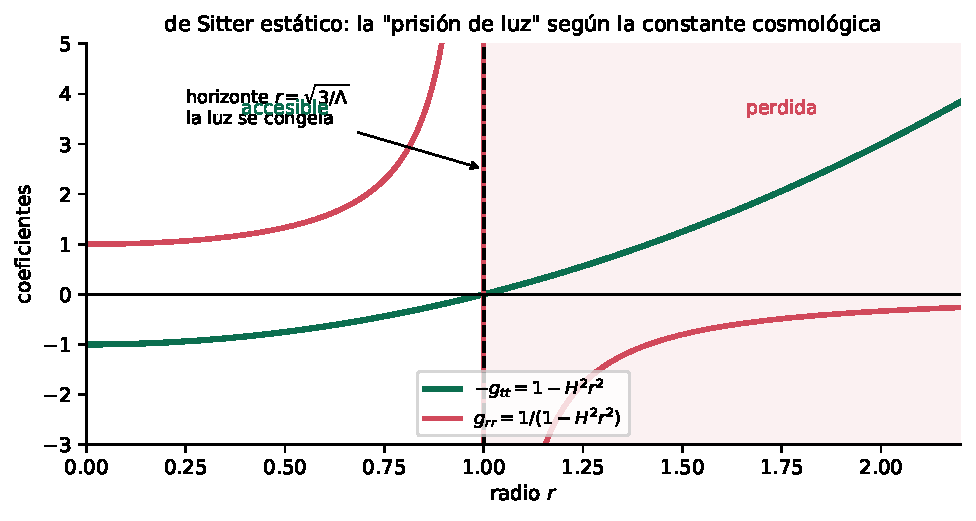
\includegraphics[width=0.72\textwidth]{desitter_estatico.pdf}
\caption{de Sitter en coordenadas estáticas: a $r=\sqrt{3/\Lambda}$ los coeficientes se anulan o explotan, señalando el horizonte cosmológico. Dentro, el observador puede comunicarse; en el horizonte, la luz ``se congela''; fuera, la región queda perdida para siempre. Cuanto mayor es $\Lambda$, menor es la prisión.}
\label{fig:desitter-estatico}
\end{figure}

\section*{Nota final: el mapa completo de la guía}

Con este último problema queda cerrado el recorrido de la geometría de Robertson--Walker, de la 2-esfera a la 3-esfera, del plasma primordial a los horizontes, y de la espuma de Kasner al interior de un agujero negro. Todos comparten el mismo hilo conductor: la métrica es la ``regla de medir'', y la cosmología es la historia de cómo esa regla cambia con el tiempo---y de qué podemos ver (y qué jamás veremos) bajo esa regla.

\end{document}
